% ---------
% --------
%!TEX TS-program = pdflatex
%!TEX encoding = UTF-8 Unicode
%!TEX spellcheck = English (Aspell)

\documentclass[11pt]{article}
\usepackage{lucy,handout,graphicx}
\usepackage{fourier-orns}
\usepackage{mathtools}
\usepackage[normalem]{ulem} % either use this (simple) or
\usepackage{tikz}

\def\Cdot{\mathbin{\text{\normalfont \textbullet}}}
\def\Sym#1{\texttt{\color{BrickRed}#1}}
\def\BlueSym#1{\textbf{\texttt{\color{RoyalBlue}#1}}}
\allowdisplaybreaks

\begin{document}

\begin{center}
\Large\textbf{CSCI 332, Fall 2026}%
\\
\LARGE\textbf{Homework 11}%
\\[0.5ex]
\large Due Monday, November 16 Anywhere on Earth (6am Tuesday)
\end{center}

\bigskip
\hrule
\bigskip

\subsection*{Submission Requirements}
\begin{itemize}
    \item Type or clearly hand-write your solutions into a PDF format so that they are legible and professional. Submit your PDF on Gradescope. 
    \item Do not submit your first draft. Type or clearly re-write your solutions for your final submission. If your submission is not legible, we will ask you to resubmit.
    \item Use Gradescope to assign problems to the correct page(s) in your solution. If you do not do this correctly, we will ask you to resubmit.
\end{itemize}

\subsection*{Academic Integrity}

Remember, you may access \EMPH{any} resource in preparing your solution to the homework. However, you \EMPH{must}
\begin{itemize}
    \item write your solutions in your own words, and
    \item credit every resource you use (for example: ``Bob Smith helped me on
    this problem. He took this course at UM in Fall 2020''; ``I found a solution
    to a problem similar to this one in the lecture notes for a different
    course, found at this link: www.profzeno.com/agreatclass/lecture10''; ``Here is a link to the full transcript of my chat with ChatGPT about the problems on this HW''.)
    Ask if you need any clarifications about how to properly cite your sources!
\end{itemize}




\newpage
%----------------------------------------------------------------------
    
\headers{CSCI 332}{Homework 11 (due November 16)}{Fall 2026}


\begin{enumerate}
%\parindent 1.5em \itemsep 4ex plus 0.5fil

%----------------------------------------------------------------------

\item (0 points) List the resources you used for each problem in this homework. If you used no resources except
lecture notes and videos and the linked textbook, you can say ``none''. If you used
an AI tool, you should put a link to your full conversation here, and you must
use the
\href{https://umaal.org/files/teaching/csci332_fall2026/agents.md}{provided
prompt}
 to guide the AI to act
as a tutor, not an answer-provider.

You will be asked to resubmit your homework if this section is blank.

Remember that no matter what resources you consulted, you must write your solutions
\emph{in your own words}.

\item (5 points)
An \emph{polygonal path} is a sequence of line segments joined end-to-end; the
endpoints of these line segments are called the vertices of the path. The
length of a polygonal path is the sum of the lengths of its segments. A
polygonal path with vertices $(x_1, y_1), (x_2, y_2),\ldots , (x_k, y_k)$ is monotonically
increasing if $x_i < x_i+1$ and $y_i < y_i+1$ for every index $i$--—informally, each
vertex of the path is above and to the right of its predecessor.

\begin{figure}[h!]
\begin{center}
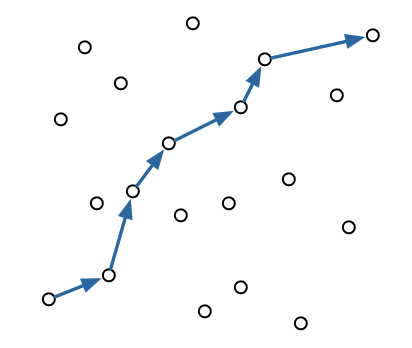
\includegraphics[width=.4\textwidth]{poly-path.png}
\end{center}
\caption{A monotonically increasing polygonal path with seven vertices through a set of points.}
\end{figure}

Suppose you are given a set $S$ of $n$ points in the plane, represented
as two arrays $X[1..n]$ and $Y[1..n]$ and an index $k$. Describe and analyze
an algorithm to compute the length of the longest
monotonically increasing path with vertices in $S$
\emph{beginning at the vertex at index k}. Assume
you have a subroutine $Length(x, y, x', y')$ that
returns the length of the segment from $(x,y)$
to $(x', y')$ in constant time.

\item (5 points) Choose any NP-Complete. To find examples, you could look
the \url{https://en.wikipedia.org/wiki/List_of_NP-complete_problems} page on Wikipedia, or you may look anywhere else
you like.
\begin{enumerate}[(a)]
    \item (2 points) In your own words, describe the problem by defining the input and the desired output. Make sure to
    frame the problem as a \emph{decision} problem.
    \item (2 point) Given an example ``yes'' instance of the problem, explain why it is a ``yes'' instance.
    (You may find examples in the literature, but please come up with your own here.)
    \item (1 point) Given an example ``no'' instance of the problem, explain why it is a ``no'' instance.
    (You may find examples in the literature, but please come up with your own here.)
    \item (4 points) Prove that the problem is in NP by giving
    \begin{enumerate}
        \item a description of a certificate that can be used to verify ``yes'' instances of the problem, and
        \item a description of a polynomial-time verification algorithm that
        takes as input an instance of the problem and a certificate, and that
        outputs ``accept'' if the instance is a ``yes'' instance
    \end{enumerate}
\end{enumerate}
Scattergories rules: if you provide a problem that is different from
every other problem submitted, you get a bonus point!
\end{enumerate}






%%%%%%%%%%%%%%%%%%%%
\end{document}
